\documentclass[10pt,journal,compsoc]{IEEEtran}
\usepackage{xeCJK}

% *** CITATION PACKAGES ***
%
\ifCLASSOPTIONcompsoc
  % IEEE Computer Society needs nocompress option
  % requires cite.sty v4.0 or later (November 2003)
  \usepackage[nocompress]{cite}
\else
  % normal IEEE
  \usepackage{cite}
\fi

\begin{document}

\title{网络游戏中收集物品的概率问题}

\author{15211068~谭伟豪~~15211063~于牧之}

\maketitle

\newtheorem{definition}{Definition}
\renewcommand{\abstractname}{摘 要}
\renewcommand{\figurename}{图}
\renewcommand{\tablename}{表}
\renewcommand{\IEEEkeywordsname}{关键词}
\begin{abstract}

  网络游戏常需要玩家收集物品, 玩家每次获得的物品往往是从一个物品池中由系统随机选取的. 对于玩家, 他们的目标常常是集齐一套物品, 但往往不了解集齐物品的难度以及自己在这个收集过程中已完成的进度. 我们通过对游戏中的收集要素进行数学建模, 从而定量地考察了一个游戏中完成收集目标的难度, 以帮助玩家更好地了解自己所玩的游戏.

\end{abstract}
\renewcommand{\abstractname}{Abstract}
\begin{abstract}
  Collecting elemnts often enter online games. In some of the games, the item that you get every time is random. Players 
\end{abstract}

\begin{IEEEkeywords}
概率, 收集式卡牌游戏.
\end{IEEEkeywords}
\renewcommand{\IEEEkeywordsname}{Keywords}
\begin{IEEEkeywords}
Probability, Collectible Card Game.
\end{IEEEkeywords}

\section{引言}

  目前市面上的网络游戏大多带有收集要素, 如地下城与勇士(DNF)中需要收集装备来提高自己的战斗力, 阴阳师中需要收集式神来优化自己的出战阵容. 对于这些游戏, 收集往往是一切的基础, 玩家只有收集到足够的物品才能体验游戏的全部内容.

  但是在这些游戏中, 玩家每次获得的物品往往是随机的. 如卡牌类游戏(CCG)中开卡包得到的卡, 大型多人在线角色扮演游戏(MMORPG)中从怪物身上获得的装备, 它们就像抽扑克牌一样具有随机性. 在这种随机性面前, 玩家往往将自己个人的所获所得归结为运气, 但从来没有对这类收集任务有一个整体的把握.

  ?? 事实上, 游戏中的收集任务远比在生活中收集东西要复杂, (如某三件物品可以构成一个套装或某十张卡牌可以构成一个卡组)

  我们从地下城与勇士这款游戏出发, 通过对游戏中的收集要素进行建模, 从而定量地考察了一个游戏中的收集任务的难度, 并在阴阳师这款卡牌游戏上成功套用了我们的模型, 体现了模型的一般性. 基于我们的模型, 我们还定义了, 从而 ??

\section{DNF中的装备收集问题}

\subsection{问题描述}

\subsection{模型建立}



\section{定义}

本节我们将探讨关于游戏中的收集任务的一些定义, 以便后续讨论. 

物品I (Item): 游戏中可获得的基本单元.

物品组G (Group): 物品构成的集合, 为游戏中发挥作用的组合单元.

候选项集C (Candidate Group): 物品组构成的集合, 物品组即其中的候选项. 对于一个候选项集, 我们只需要获得其中的一个物品组即可满足收集目标. 

目标集T (Target): 候选项集构成的集合.

目标的完成: 
对于目标集$T = \{C_1, C_2, \dots, C_n\}$和已收集的物品集合$S$, 如果$\exists \{G_{k_1}, G_{k_2}, \dots, G_{k_n} | G_{k_i} \in C_i\} \subseteq S$, 则称收集目标完成了.


为了便于理解, 我们以DNF这款游戏为例来阐述上述概念.

物品: $I_1$=皮夹肩甲, $I_2$=皮夹上衣, $I_3$=皮夹裤子, $I_4$=皮夹腰带, $I_5$=皮夹鞋子, $I_6$=轻甲肩甲, $I_7$=轻甲上衣, $I_8$=轻甲裤子, $I_9$=轻甲腰带, $I_{10}$=轻甲鞋子, $I_{11}$=太刀, $I_{12}$=巨剑, $I_{13}$=手镯, $I_{14}$=项链, $I_{15}$=戒指, $I_{16}$=辅助装备, $I_{17}$=魔法石, $I_{18}$=耳环. 

物品组: 皮夹套$G_1=\{I_1, I_2, I_3, I_4, I_5\}$, 轻甲套$G_2=\{I_6, I_7, I_8, I_9, I_{10}\}$, 太刀$G_3=\{I_{11}\}$, 巨剑$G_4=\{I_{12}\}$, 首饰套$G_5=\{I_{13}, I_{14}, I_{15}\}$, 辅助装备$G_6=\{I_{16}\}$, 魔法石$G_7=\{I_{17}\}$, 耳环$G_8=\{I_{18}\}$.

候选项集: 衣服$C_1=\{G_1, G_2\}$, 武器$C_2=\{G_3, G_4\}$, 首饰$C_3=\{G_5\}$, 辅助装备$C_4=\{G_6\}$, 魔法石$C_5=\{G_7\}$, 耳环$C_6=\{G_8\}$

目标集: $T=\{C_1, C_2, C_3, C_4, C_5, C_6\}$

目标的完成: 玩家获得了皮夹套和轻甲套之一, 太刀和巨剑之一, 首饰套, 辅助装备, 魔法石, 耳环. 


\section{模型的建立}

针对上面的研究问题, 我们可以对迁移学习的情境和方法进行分类. 

\begin{table*}[!ht]
\centering
\caption{迁移学习的方法}
\label{tab:survey_method}
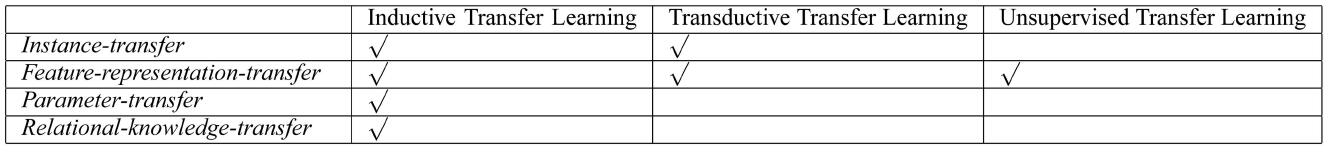
\includegraphics[width=40pc]{img/survey_tab3.jpg}
\end{table*}

\begin{figure*}[!ht]
\centering
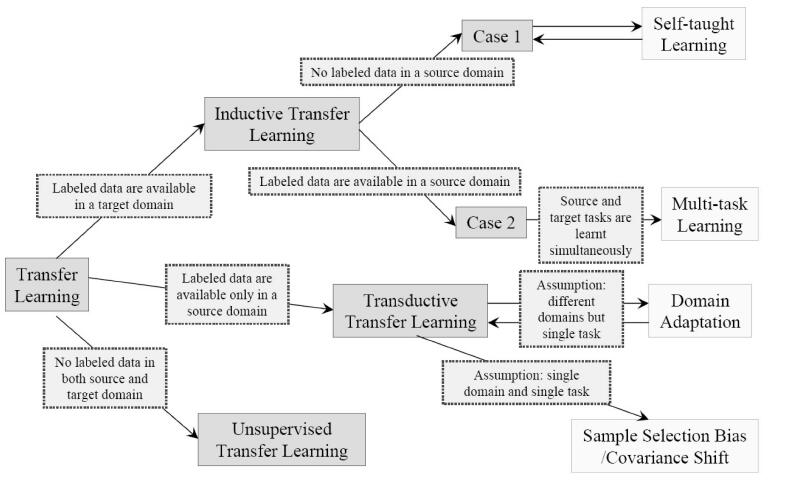
\includegraphics[width=30pc]{img/survey_fig1.jpg}
\caption{迁移学习方法与情境的关系}
\label{fig:survey_method}
\end{figure*}


\begin{enumerate}
\item 在归纳迁移的情境中, 目标任务和源任务是不同的, 而目标域和源域可能相同也可能不同. 此类问题中, 目标域中必须要有带标签的数据才能训练出目标预测模型$f_T(\cdot)$. 根据源域中无标签数据和标签数据的情形不同, 我们还能进一步将归纳迁移算法分为这样两类:\\
a. 源域中有很多标签数据. 此时归纳迁移算法类似于多任务学习算法. 但区别在于, 前者更侧重于在目标问题中取得更好的性能, 而后者则试图同时完成源任务和目标任务. \\
b. 源域中无标签数据. 此时归纳学习算法比较接近自学(self-taught learning)算法. 因为在自学算法的使用场景中源任务和目标任务的标签空间可能不同, 而这与源域中无标签数据的情形是很近似的. 

\item 在转导学习的情境中, 目标任务和源任务是一样的, 但源域和目标域是不同的. 这种情况下目标域是没有标签数据的, 但源域有很多. 根据源域和目标域之间的区别, 我们还能进一步将转到学习的情境划分为这样两类:\\
a. 二者的特征空间不同$X_S \ne X_T$\\
b. 特征空间相同$X_S \ne X_T$, 但边缘概率分布不同, $P(X_S) \ne P(X_T)$\\
后者和文本分类中的域适应很相似, 因为他们的基本假设是一样的. 
\item 最后, 还有无监督迁移学习的情境. 它与归纳迁移学习的情境类似, 目标问题和源问题不同但相关. 区别在于, 无监督迁移学习中目标问题是无监督问题, 如聚类、降维等. 在此情境中, 源域和目标域都没有带标签的数据. 
\end{enumerate}




\section{结论}

地下城与勇士没有妹子好玩. 

\bibliographystyle{IEEEtran}
\bibliography{thesis}

\end{document}
